\documentclass[notes]{beamer}          % print frame + notes
%\documentclass[notes=only]{beamer}     % only notes
%\documentclass{beamer}                 % only frames

\usecolortheme{beaver}

% Some commonly used packages
% (copied mainly from the Utrecht University theme: https://www.overleaf.com/project/5c900fa3bd9930036341116a)
\usepackage{ragged2e}  % `\justifying` text
\usepackage{booktabs}  % Tables
\usepackage{tabularx}
\usepackage{tikz}      % Diagrams
\usetikzlibrary{calc, shapes, backgrounds}
\usepackage{amsmath, amssymb, amsfonts, amsthm}
\usepackage{url}       % `\url`s
\usepackage{listings}  % Code listings
\usepackage{comment}
\usepackage{mathtools}
\usepackage{graphicx}
\usepackage{subfig}
\usepackage{bm}

% Mainly math commands
\newcommand{\vect}[1]{\bm{#1}}
\usepackage{amsfonts}% to get the \mathbb alphabet
\newcommand{\field}[1]{\mathbb{#1}}
\newcommand{\C}{\field{C}}
\newcommand{\R}{\field{R}}
\newcommand{\norm}[1]{\left\lVert#1\right\rVert}
\newcommand{\argmin}{\operatornamewithlimits{argmin}}
\providecommand{\abs}[1]{\lvert#1\rvert}
\providecommand{\norm}[1]{\lVert#1\rVert}

% Bibliography
\usepackage[uniquename=init,giveninits=true,maxcitenames=1,style=authortitle-comp]{biblatex}
\bibliography{lectures/references}

\setbeamertemplate{section in toc}{\inserttocsectionnumber.~\inserttocsection}


%Information to be included in the title page:
\title{Machine learning foundations I}
\author{Mitko Veta}
\institute{Eindhoven University of Technology

Department of Biomedical Engineering}
\date{2019}



\begin{document}

\frame{\titlepage}


\begin{frame}
\frametitle{Learning goals}

At the end of this lecture you will:
\begin{itemize}
    \item Have an understanding of the goal of machine learning (ML) models.
    \item Have a good understanding of basic mathematical concepts used in ML and be able to apply them in the design and implementation of ML methods.
\end{itemize}
\end{frame}

\begin{frame}{Overview}
Topics covered in this lecture:
    \tableofcontents
\end{frame}

\section{Linear algebra}

\begin{frame}
\frametitle{Linear algebra}
Materials:
\begin{itemize}
    \item Chapter I.2 from \cite{deeplearning}
    \item \cite{linearalgebra}
\end{itemize}

\end{frame}

\begin{frame}
\frametitle{Scalars}
\begin{itemize}
    \item A scalar is a single number (integer, real, rational, ...).
    \item Denoted by italics $a, n, x$

\end{itemize}
\end{frame}

\begin{frame}
\frametitle{Vectors}
\begin{itemize}
    \item A vector is a 1-D array of numbers (integer, real, rational, ...)
    $
    \vect{x} = \begin{bmatrix} x_1 \\ x_2 \\ \ldots \\ x_n \end{bmatrix}
    $
    \item{Example notation for type and size} \\
    $\vect{x} \in \R^n$
 \end{itemize}
\end{frame}


\begin{frame}
\frametitle{Matrices}
\begin{itemize}
    \item A matrix is a 2-D array of numbers \\
    $$
    \begin{bmatrix}
    a_{1,1} & a_{1,2} \\
    a_{2,1} & a_{2,2}
    \end{bmatrix}
    $$
    \item Example notation for type and shape \\
    $\mathbf{A} \in \R^{m \times n}$
\end{itemize}
\end{frame}

\begin{frame}
\frametitle{Tensors}
\begin{itemize}
    \item A tensor is an array of numbers that may have
    \begin{itemize}
        \item a zero dimensions and be a scalar,
        \item one dimension and be a vector,
        \item two dimensions and be a matrix,
        \item more dimensions ...
    \end{itemize}
\end{itemize}

{\bf Side note}: One of the most popular frameworks for implementing deep machine learning models is called TensorFlow (https://www.tensorflow.org/).

\end{frame}

\begin{frame}
\frametitle{Transpose matrix}
    %\begin{itemize}
         $$(\vect{A}^T)_{i,j} = \vect{A}_{j,i}$$

        $$ \vect{A} = \begin{bmatrix}
                        A_{1,1} & A_{1,2}  \\
                        A_{2,1} & A_{2,2}  \\
                        A_{3,1} & A_{3,2}
                      \end{bmatrix} \Rightarrow
                      \begin{bmatrix}
                        A_{1,1} & A_{2,1} & A_{3,1} \\
                        A_{1,2} & A_{2,2} & A_{3,2}
                      \end{bmatrix}
                      $$
        The transpose matrix is a mirror image with regard to the main diagonal \\
        $$(\vect{A}\vect{B})^T = \vect{B}^T\vect{A}^T$$
    %\end{itemize}

\end{frame}

\begin{frame}
\frametitle{Identity matrix}
    \begin{itemize}
        \item Identity matrix $\vect{I}_3$
        $$\begin{bmatrix}
            1 & 0 & 0 \\
            0 & 1 & 0 \\
            0 & 0 & 1
          \end{bmatrix}$$

        \item The identity matrices are neutral elements in matrix-matrix and matrix-vector multiplication, e.g.
        $$\forall \vect{x} \in \R^n: \vect{I}_n \vect{x} = \vect{x} \vect{I}_n = \vect{x} $$
    \end{itemize}

\end{frame}

\begin{frame}
\frametitle{Matrix (dot) product}

    $$\vect{C} = \vect{A}\vect{B}$$
    The matrices must be compatible: an $m \times n$ matrix is multiplied with an $n \times r$ matrix and as a result an $m \times r$ matrix is obtained
    $$C_{i,j} = \sum_k A_{i,k}B_{k,j}$$

    $$
    \vect{A}
    \begin{bmatrix}
       1 & 2 & 3 \\
       4 & 5 & 6 \\
       7 & 8 & 9 \\
       10 & 11 & 12
    \end{bmatrix}
    \times
    \vect{B}
    \begin{bmatrix}
        1 & 2 & 3 & 4 & 5 \\
        6 & 7 & 8 & 9 & 10 \\
        11 & 12 & 13 & 14 & 15
    \end{bmatrix} =
    \vect{C}
    \begin{bmatrix}
       4 \times 5
    \end{bmatrix}
    $$
    $$ C_{2,5} = A_{2,1}B_{1,5} + A_{2,2}B_{2,5} + A_{2,3}B_{3,5} = 4 \cdot 5 + 5 \cdot 10 + 6 \cdot 15 = 160 $$

\end{frame}

\begin{frame}{Matrix (dot) product}
    \begin{itemize}
        \item In general matrix multiplication is not commutative, i.e., most of the time $\vect{A}\vect{B} \not = \vect{B}\vect{A}$.
        \item Depending on the dimensions sometimes $\vect{A} \vect{B}$ or $\vect{B} \vect{A}$ are not possible.
        \item As a special case the matrix can be a (column or row) vector; an $m \times n$ matrix is multiplied with a $n \times 1$ vector to obtain a $m \times 1$ vector.
    \end{itemize}
\end{frame}


\begin{frame}
\frametitle{Systems of equations}
    \begin{itemize}
        \item $\vect{A}\vect{x} = \vect{b}$ expands to
        \begin{center}
        \begin{align}
            \vect{A}_{1,:} \vect{x}_1 = \vect{b}_1 \\
            \vect{A}_{2,:} \vect{x}_2 = \vect{b}_2 \\
            \ldots \\
            \vect{A}_{m,:} \vect{x}_m = \vect{b}_m
        \end{align}
        \end{center}
    \end{itemize}

\end{frame}




\begin{frame}
\frametitle{Solving systems of linear equations}
    \begin{itemize}
        \item A linear system of equations can have
            \begin{itemize}
                \item no solutions,
                \item many solutions,
                \item exactly one solution.
            \end{itemize}
        \item Only one solution implies that multiplication by a matrix is an invertible operation.
    \end{itemize}

\end{frame}

\begin{frame}
\frametitle{Matrix inversion}
    \begin{itemize}
        \item Matrix inverse is defined with
            $$ \vect{A}^{-1}\vect{A} = \vect{I}_n $$
        \item A system of linear equations can be solved using inverse matrix
        \begin{center}
            $$ \vect{A} \vect{x} = \vect{b} $$
            $$ \vect{A}^{-1}\vect{A} \vect{x} = \vect{A}^{-1}\vect{b} $$
            $$ \vect{I}_n \vect{x} = \vect{A}^{-1}\vect{b} $$
            $$ \vect{x} = \vect{A}^{-1}\vect{b} $$
        \end{center}
        \item This is useful mostly for abstract analysis.
        \item From a numerical point of view there are much more efficient methods.
    \end{itemize}
\end{frame}


\begin{frame}
\frametitle{Invertibility}
    A matrix cannot be inverted if
    \begin{itemize}
        \item the number of rows and columns is not the same, or
        \item some rows and columns are "redundant" ("linearly dependent", "low rank").
    \end{itemize}
\end{frame}

\begin{frame}
\frametitle{Norms}
    \begin{itemize}
        \item Norms are functions that measure how "large" a vector is.
        \item Similar to a distance between zero and the point represented by the vector
        \begin{itemize}
           \item $f(\vect{x}) = 0 \Rightarrow \vect{x} = 0$
           \item $f(\vect{x} + \vect{y}) \leq f(\vect{x}) + f(\vect{y})$ (\bf the triangle inequality)
           \item $\forall \alpha \in \R: f(\alpha \vect{x}) = \alpha f(\vect{x})$
        \end{itemize}
    \end{itemize}
\end{frame}

\begin{frame}
\frametitle{Norms}
    \begin{itemize}
        \item $L^p$- norm
        $$\norm{\vect{x}}_p = \left( \sum_i |x_i|^p  \right) ^{\frac{1}{p}}$$
        \begin{itemize}
            \item Most popular $L^2$-norm (for $p=2$)
            \item $L_1$-norm (for $p = 1$): $\norm{\vect{x}}_1 = \sum_i |x_i|$
            \item Max norm (for infinite $p$): $\norm{\vect{x}}_\infty = \max_i |x_i|$
            \end{itemize}
    \end{itemize}

\end{frame}

\begin{frame}
\frametitle{Special vectors and matrices}
    \begin{itemize}
        \item Unit vector $\norm{\vect{x}}_n = 1$
        \item Symmetric matrix $\vect{A} = \vect{A}^T$
        \item Orthogonal matrix $$\vect{A}\vect{A}^T = \vect{I} = \vect{A}^T \vect{A}$$
        \item It follows that for orthogonal matrices  $\vect{A}^T = \vect{A}^{-1}$
    \end{itemize}
\end{frame}

\begin{frame}
\frametitle{Eigendecomposition}
    \begin{itemize}
        \item Eigenvector and eigenvalue
        $$ \vect{A}\vect{x} = \lambda \vect{x}$$
        \item Eigendomdecomposition of a diagonazible matrix
        $$ \vect{A} = \vect{A} \mbox{diag}(\lambda) \vect{A}^{-1}$$
        where $\mbox{diag}(\lambda)$ is a diagonal matrix having the (scalar) eigenvalues $\lambda$ as diagonal elements.
    \end{itemize}

\end{frame}

\begin{frame}
\frametitle{Eigendecomposition}
    \begin{itemize}
        \item Every real symmetric matrix has a real orthogonal eigendecomposition
        $$ \vect{A} = \vect{Q} \vect{\Lambda} \vect{Q}^T $$
        where $\vect{Q}$ is an orthogonal matrix composed of eigenvectors of $\vect{A}$ and $\vect{\Lambda}$ is a diagonal matrix.
        \item The eigenvalue $\Lambda_{ii}$ is associated with the eigenvector in column $i$ of $\vect{Q}$, denoted as $\vect{Q}_{:,i}$.
        \item We can think of $\vect{A}$ as scaling space by factor $\lambda_i$ in the direction of its corresponding eigenvector $v^{(i)}$ (represented by $\vect{Q}_{:,i}$).
    \end{itemize}

\end{frame}

\begin{frame}
\frametitle{Eigendecomposition}
    \begin{itemize}
        \item From the eigendecomposition we learn useful properties of the matrix.
        \item The eigendecomposition of a real symmetric matrix is used in optimization of quadratic expressions of the form $f(\vect{x}) = \vect{x}^T \vect{A} \vect{x}$ under the constraint $\norm{\vect{x}}_2 = 1$.
        \item For instance, if $\vect{x}=\vect{v}^{(i)}$, then $f(\vect{x}) = \lambda_i$, when $\vect{v}^{(i)}$ is an eigenvector of $A$ and $\lambda_i$ is its corresponding eigenvalue.
        \item The maximal (minimal) value of $f$ within the constraint region is equal to the maximal (minimal) eigenvalue.
    \end{itemize}

\end{frame}


\begin{frame}
\frametitle{Effect of eigenvalues}

\begin{center}
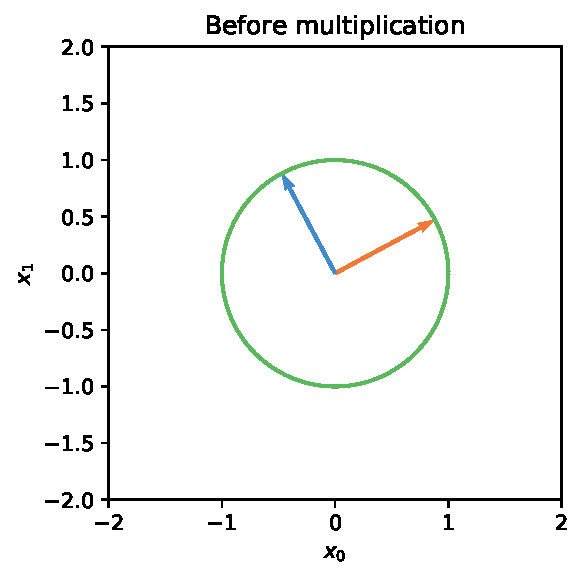
\includegraphics[width=0.5\textwidth]{figures/week_1/unit_circle_before.pdf}
\hfill
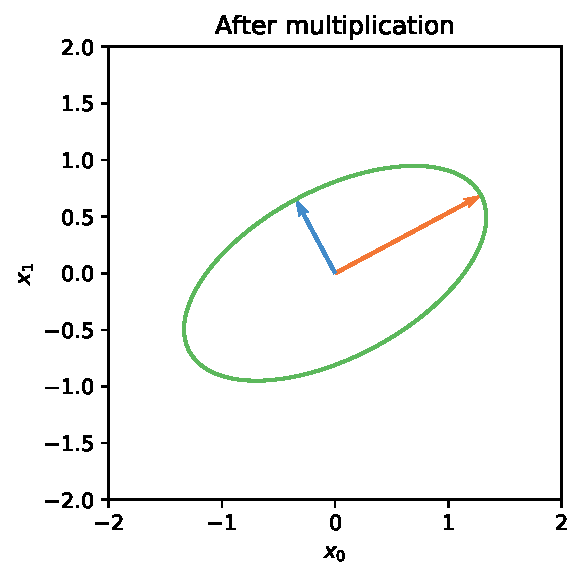
\includegraphics[width=0.5\textwidth]{figures/week_1/unit_circle_after.pdf}
\end{center}

\end{frame}


\begin{frame}
\frametitle{Singular value decomposition}
    \begin{itemize}
        \item Similar to eigenvalue decomposition
        \item More general: matrix need not be square
        $$\vect{A} = \vect{U} \vect{D} \vect{V}^T$$
        \item $\vect{U}$ and $\vect{V}$ are square matrices and are both orthogonal, $\vect{D}$ is diagonal.
        \item The diagonal elements of $D$ are called {\bf singular values} of matrix $\vect{A}$; the columns of $\vect{U}$ and $\vect{V}$ are {\bf left-singular} and {\bf right-singular vectors} of $\vect{A}$, respectively.
    \end{itemize}

\end{frame}

\begin{frame}
\frametitle{Moore-Penrose pseudoinverse}
    \begin{itemize}
        \item Matrix inversion is not defined on matrices that are no square.
        \item The {\bf Moore-Penrose pseudoinverse} is defined as
        $$
        \vect{A}^{+} = \lim_{\alpha \searrow 0}(\vect{A}^T\vect{A}+\alpha \vect{I})^{-1}\vect{A}^T
        $$

    \end{itemize}
\end{frame}

\begin{frame}
\frametitle{Moore-Penrose pseudoinverse}
    Now we can consider
    $$\vect{x} = \vect{A}^{+} \vect{y}$$
    \begin{itemize}
        \item If the equation has
            \begin{itemize}
                \item exactly one solution: this is the same as inverse,
                \item no solution: gives the solution with the smallest error, $\norm{\vect{A}\vect{x} - \vect{y}}_2$
                \item many solutions: gives the solution with the smallest norm of $\vect{x}$.
            \end{itemize}
    \end{itemize}

\end{frame}

\begin{frame}
\frametitle{Computing the pseudoinverse}
    \begin{itemize}
        \item Efficient implementations are based on the formula allowed by the singular decomposition
        $$
        \vect{A}^{+} = \vect{V}\vect{D}^{+}\vect{U}^T
        $$
        \item $\vect{U},\vect{D},\vect{V}$ are from the singular value decomposition.
        \item The pseudoinverse $\vect{D}^{+}$ of $\vect{D}$ is obtained by taking the reciprocal non-zero elements and after that taking the transpose of the resulting matrix.
    \end{itemize}

\end{frame}

\begin{frame}
\frametitle{Trace}
    \begin{itemize}
        \item A {\bf trace} of a matrix is defined as
        $$Tr(\vect{A}) = \sum_{i} \vect{A}_{i,i} $$
        \item Expressions in terms of the trace operators allow to exploit many useful identities, e.g.
        $$Tr(\vect{A}\vect{B}\vect{C}) = Tr(\vect{B}\vect{C}\vect{A}) = Tr(\vect{C}\vect{A}\vect{B})$$
    \end{itemize}

\end{frame}

\section{Gradient-based optimization}


\begin{frame}
\frametitle{Gradient-based optimization}
Materials:
\begin{itemize}
    \item Chapters I.4 and I.5 from \cite{deeplearning}
    \item \cite{linearalgebra}
\end{itemize}
\end{frame}

\begin{frame}
\frametitle{Gradient}
    \begin{itemize}
        \item Let $f: \R^{m \times n} \mapsto \R$ be a function that takes $m \times n$ matrix $\vect{A}$ as input and returns a real number (scalar).
        \item A {\bf gradient} of $f$ with respect to $A$ is the matrix
        $$
        \nabla_{\vect{A}} f(\vect{A}) =
        \begin{bmatrix}
         \frac{\partial f}{\partial A_{11}} & \frac{\partial f}{\partial A_{12}} & \ldots & \frac{\partial f}{\partial A_{1n}} \\
          \frac{\partial f}{\partial A_{21}} & \frac{\partial f}{\partial A_{22}} & \ldots & \frac{\partial f}{\partial A_{2n}} \\
          \vdots & \vdots & \ddots & \vdots \\
           \frac{\partial f}{\partial A_{m1}} & \frac{\partial f}{\partial A_{m2}} & \ldots & \frac{\partial f}{\partial A_{mn}}
        \end{bmatrix}
        $$
        \item i.e. an $m \times n$ matrix with  $$(\nabla_{\vect{A}} f(\vect{A}))_{ij} = \frac{\partial f}{\partial A_{ij}}  $$
        \item The size of the gradient of $\vect{A}$ is the same as the size of $A$.

    \end{itemize}
\end{frame}

\begin{frame}
\frametitle{Gradient}
    \begin{itemize}
        \item In the special case when $A$ is a vector we obtain the (possibly more familiar) gradient
        $$ \nabla_{\vect{x}} f(\vect{x}) =
        \begin{bmatrix}
         \frac{\partial f}{\partial x_{1}}  \\
          \frac{\partial f}{\partial x_{2}}  \\
          \vdots  \\
           \frac{\partial f}{\partial x_{m}}
        \end{bmatrix}$$
        \item In general to define a gradient we require that the function returns a {\bf real} value.
    \end{itemize}

\end{frame}

\begin{frame}
\frametitle{Jacobian}

\begin{itemize}
    \item The Jacobian $\vect{J_f}$ is a generalization of the gradient for vector valued functions.
    \item Let $\vect{f}:\R^n \mapsto \R^m $ be a function that takes $n$-dimensional vector $\vect{x}$ as input and returns a $m$-dimensional vector as an output.
    \item The Jacobian $\vect{J_f}$ is defined as
    $$
        \vect{J_f} =
        \begin{bmatrix}
         \frac{\partial f_1}{\partial x_{1}} & \frac{\partial f_1}{\partial x_{2}} & \ldots & \frac{\partial f_1}{\partial x_{n}} \\
          \frac{\partial f_2}{\partial x_{1}} & \frac{\partial f_2}{\partial x_{2}} & \ldots & \frac{\partial f_2}{\partial x_{n}} \\
          \vdots & \vdots & \ddots & \vdots \\
           \frac{\partial f_m}{\partial x_{1}} & \frac{\partial f_m}{\partial x_{2}} & \ldots & \frac{\partial f_m}{\partial x_{n}}
        \end{bmatrix}
    $$
    \item Note that for the special case of a scalar-valued function, the Jacobian is the transpose of the gradient.
\end{itemize}

\end{frame}

\begin{frame}
\frametitle{Optimization}

\begin{itemize}
    \item Most machine learning methods involve some kind of optimization.
    \begin{itemize}
        \item One exception is the $k$-Nearest neighbour classifier introduced later.
    \end{itemize}
    \item Optimization means minimizing or maximizing some function $f(\vect{x})$, i.e. finding the values of $\vect{x}$ for which $f(\vect{x})$ has a minimum or a maximum.
    \item Notation: $\vect{x}^* = \argmin f(\vect{x})$
\end{itemize}
\end{frame}


\begin{frame}{Gradient-based optimization}

\begin{itemize}
    \item The derivative tells us how to change $x$ in order to make a small improvement of $f(x)$.
    \item Therefore, derivatives can be useful in optimization.


\end{itemize}
\end{frame}


\section{Two simple machine learning models}


\begin{frame}
\frametitle{Two simple machine learning models}
Materials:
\begin{itemize}
    \item Chapter 2.3 from \cite{elements}
\end{itemize}

\end{frame}

\begin{frame}
\frametitle{Some notations}
    \begin{itemize}
        \item We denote an input variable with the symbol $x$ (scalar) or $\vect{x}$ (vector).
        \item The $i$-th component of a vector input $\vect{x}$ is denoted as $x_i$.
        \item Quantitative (numerical) outputs are denoted with $y$.
        \item Qualitative outputs are denoted with $g$ (from group) and take values from a set $\cal{G}$.
        \item Matrices are denoted with bold and uppercase letters $\vect{X}$\\
        for instance, a set of $N$ input $p$-vectors $\vect{x}_i$ ($1 \leq i \leq N)$ is "packed" in a $N \times p$ input matrix $\vect{X}$.
        \item Since by default vectors are assumed to be column vectors, the rows of $\vect{X}$ are the transposes $\vect{x}_i^T$.
    \end{itemize}
\end{frame}

\begin{frame}
\frametitle{The learning task}
    \begin{itemize}
        \item Given a value of the input vector $\vect{x}$ make a good prediction of the output $y$, denoted as $\hat{y}$.
        \item Both $y$ and $\hat{y}$ should take values from the same numerical set.
        \item Similarly, $g$ and $\hat{g}$ should both take values from the same set $\cal{G}$.
         \item We suppose that we have available a set of measurements $(\vect{x}_i,y_i)$ or $(\vect{x}_i,g_i)$ $(1 \leq i \leq N)$ called {\bf training data} \\
         (in matrix form: $(\vect{X},\vect{y})$ and/or $(\vect{X},\vect{g})$).
        \item Our task is to construct a prediction rule based on the training data.

    \end{itemize}

\end{frame}


\begin{frame}
\frametitle{The learning task}
    Example:
    \begin{itemize}
         \item {\bf Variable values}: Let $g$ (and therefore also $\hat{g}$) be two valued (categorical), e.g. $\cal{G} = \{ \text{\textcolor{blue}{BLUE}, \textcolor{orange}{ORANGE}}\}$.
        \item {\bf Encoding of $g$s with $y$s}: Then each class can be encoded binary, i.e., with $y \in \{0,1\}$, e.g., \textcolor{blue}{BLUE} and \textcolor{orange}{ORANGE}, would correspond to $0$ and $1$, respectively.
        \item {\bf Predicted output values}: $\hat{y}$ ranges over the interval $[-\infty,+\infty]$ (of which $\{0,1\}$ is a subset).
        \item {\bf Prediction rule}: $\hat{g}$ is assigned a (class label) \textcolor{blue}{BLUE} if $\hat{y} < 0.5$ and \textcolor{orange}{ORANGE}, otherwise.

    \end{itemize}
\end{frame}



\begin{frame}
\frametitle{Two simple approaches to prediction}
\begin{itemize}
    \item Linear model fit
        \begin{itemize}
            \item strong assumptions about the structure of the decision boundary
            % \item stable but possibly inaccurate predictions
        \end{itemize}
    \item $k$-nearest neighbours
        \begin{itemize}
            \item weak assumptions about the structure of the decision boundary
            % \item predictions most often accurate but possibly unstable
        \end{itemize}
\end{itemize}

\end{frame}

\subsection{Linear model}

\begin{frame}
\frametitle{Linear model fit by least squares}
    \begin{itemize}
        \item Despite relative simplicity one of the most important statistical tools
        \item Input vector $\vect{x}^T = (x_1, x_2, \ldots, x_p)$
        \item Output $y$ predicted using the model \\
            \begin{center}
            $\hat{y} = \hat{w_0} + \sum_{j=1}^{p} x_j \hat{w_j}$
            \end{center}
        \item $\hat{w}_i$ $ (0 \leq i \leq p)$ are the parameters of the linear model
        \item In vector form
            \begin{center}
            $\hat{y} = \hat{\vect{w}}^T\vect{x} = \vect{x}^T \hat{\vect{w}}$
            \end{center}
            using the fact that the scalar (inner) product of two vectors is a commutative operation
    \end{itemize}
\end{frame}

\begin{frame}
\frametitle{Linear model fit by least squares}
    \begin{itemize}
        \item  We assume that $w_0$ is in $\vect{w}$ and $1$ is included in $\vect{x}$.
        \item $\hat{y}$ is a scalar, but in general can be a $k$-vector $\hat{\vect{y}}$, in which case $\vect{w}$ becomes a $p \times k$ matrix of coefficients.
    \end{itemize}
\end{frame}

\begin{frame}
\frametitle{Linear model fit by least squares}
    Some hyper(space) terminology:
    \begin{itemize}
        \item Points $\vect{x},\hat{y}$ form a {\bf hyperplane} in the $(p+1)$-dimensional input-output hyperspace.
        \item If $\vect{x}$ is extended with constant $1$ then the hyperplane includes the origin and it forms a {\bf subspace}.
        \item If $1$ is not included then the hyperplane is an {\bf affine} set and it cuts the $y$-axis at the point $(\vect{0}, \hat{w_0})$, where the vector $\vect{0}$ has all $x_i$ coordinates equal to $0$.
        \item Reminder: from now on we assume that $1$ is included in $\vect{x}$ and $\hat{w_0}$ in $\hat{\vect{w}}$
        \item The function $f(\vect{x}) =  \vect{w}^T \vect{x}$ defined on the $p$-dimensional (input) space is a {\bf linear} function (we omit the hats over the $w$s since now we consider them as free variables)
        \item The gradient $\nabla f(\vect{x})$ is a vector pointing along the direction of maximal change.
    \end{itemize}

\end{frame}


\begin{frame}
\frametitle{Linear model fit by least squares}
\frametitle{}
    \begin{itemize}
        \item There are many ways to fit a linear model to a training dataset.
        \item {\bf Least squares} method
            \begin{itemize}
                \item We need to find coefficients $\hat{w_i}$ which minimize the error estimated with the {\bf residual sum of squares}
                \begin{center}
                    $$\mbox{RSS}(\vect{w}) = \sum_{i = 1}^{N}(y_i - \vect{x}_i^T \vect{w})^2$$
                \end{center}
                 assuming $N$ input-output pairs.
            \end{itemize}
        \item $\mbox{RSS}(\vect{w})$ is a quadratic function.
        \item A minimum always exists though not necessarily a unique one.
    \end{itemize}

\end{frame}


\begin{frame}
\frametitle{Linear model fit by least squares}
    \begin{itemize}
        \item We look for the solution $\hat{\vect{w}}$ using the matrix notation:
        \item $\vect{y} = [y_1, y_2, \ldots, y_N]^T$ is the vector formed from the $N$ output vectors and $\vect{X}$ is an $N \times p$ matrix  \\
        % (\vect{y} - \vect{X}^T \vect{w})^2 =
        $$\mbox{RSS}(\vect{w}) =  (\vect{y} - \vect{X} \vect{w})^T (\vect{y} - \vect{X} \vect{w})$$
        \item To find the minimum we differentiate with respect to $\vect{w}$ which gives
        $$(-\vect{X})^T(\vect{y}-\vect{X}\vect{w}) + (\vect{y}-\vect{X}\vect{w})^T (-\vect{X})$$
        using the rule $(\vect{A}\vect{B})^T = \vect{B}^T\vect{A}^T$ this is equivalent to
        $$ -2 \vect{X}^T(\vect{y}-\vect{X}\vect{w})$$
    \end{itemize}
\end{frame}

\begin{frame}
\frametitle{Linear model fit by least squares}
    \begin{itemize}

    \item To find the minimum our derivative must be $\vect{0}$, hence:
        $$\vect{X}^T(\vect{y}-\vect{X}\vect{w}) =  \vect{0}$$
        $$\vect{X}^T \vect{y} -\vect{X}^T\vect{X}\vect{w} =  \vect{0}$$
        $$ \vect{X}^T \vect{y} = \vect{X}^T\vect{X}\vect{w}$$
    \item    If $\vect{X}^T\vect{X}$ is non-singular there exists a unique solution given by
        $$\hat{\vect{w}} = (\vect{X}^T\vect{X})^{-1}\vect{X}^T \vect{y}$$
    \end{itemize}

         {\bf Question}: Why not simply $\vect{y} -\vect{X}\vect{w}=  \vect{0}$ $\rightarrow$ $\vect{y} = \vect{X}\vect{w}$ $\rightarrow$ $\hat{\vect{w}} = \vect{X}^{-1} \vect{y}$?

\end{frame}


\begin{frame}{Linear model fit by least squares}
    \begin{itemize}
        \item For each input $\vect{x}_i$ there corresponds the fitted output $$\hat{y}_i = \hat{y}_i(\vect{x}_i) = \hat{\vect{w}}^T\vect{x}_i$$.
        \item This is called ``making a prediction'' for $\vect{x}_i$.

        \item The entire fitted surface (hyperplane) is fully characterized by the parameter vector $\hat{\vect{w}}$.

        \item After fitting the model, we can ``discard'' the training dataset.
    \end{itemize}
\end{frame}

\begin{frame}
\frametitle{Example: Linear model fit by least squares}
\begin{itemize}
    \item Scatter plot of training data on a pair of inputs $x_1$ and $x_2$
    \item Output class variable $g$ has two values \textcolor{blue}{BLUE} and \textcolor{orange}{ORANGE}.
    \item Linear regression model fitted with the response variable $y$ coded as $0$ for \textcolor{blue}{BLUE} and $1$ for \textcolor{orange}{ORANGE}.
    \item Fitted values $\hat{y}$ converted to a fitted class variable $\hat{g}$ as
    \[ \hat{g} = \begin{cases}
                    \text{\textcolor{blue}{BLUE}}  & \text{if $\hat{y} \leq 0.5$} \\
                    \text{\textcolor{orange}{ORANGE}} & \text{if $\hat{y} > 0.5$ }
                 \end{cases} \]

\end{itemize}
\end{frame}

\begin{frame}{Example: Linear model fit by least squares}
    \begin{center}
        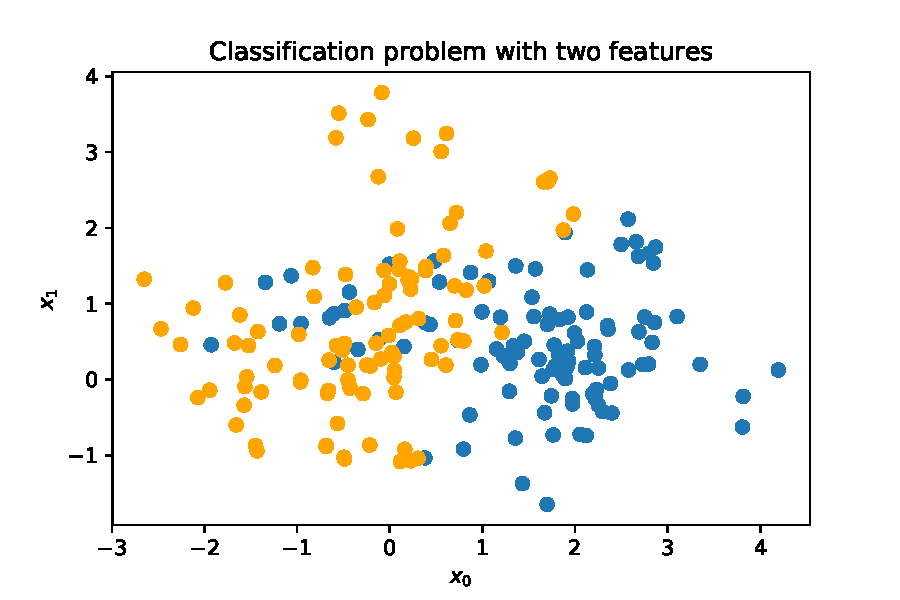
\includegraphics[width=0.5\textwidth]{figures/week_1/classification_problem.pdf}
        \hfill
        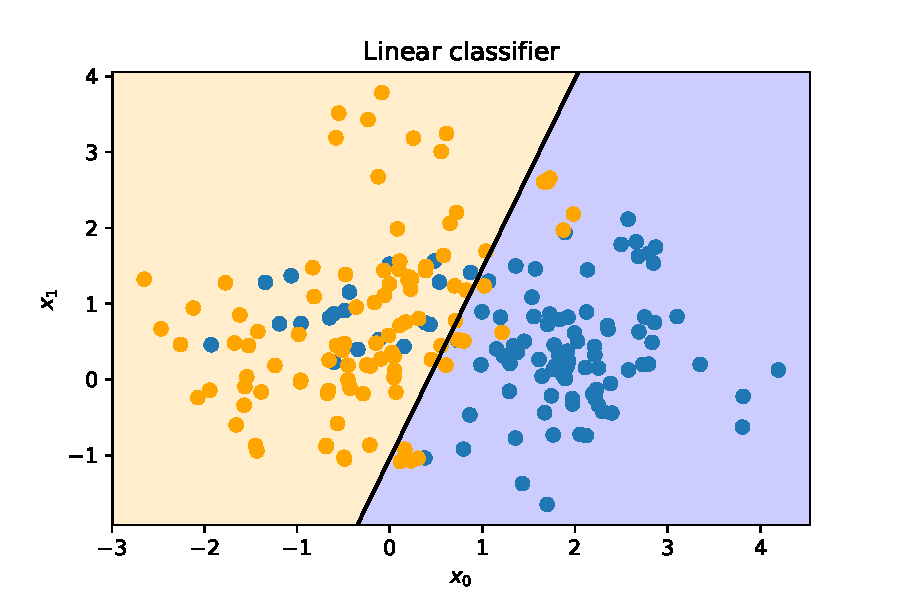
\includegraphics[width=0.5\textwidth]{figures/week_1/linear_model.pdf}
        \end{center}
\end{frame}


\begin{frame}
\frametitle{Example: Linear model fit by least squares}
\begin{itemize}
    \item Two classes separated in the plane ($\R^2$) by the decision boundary $\{ \vect{x} : \vect{w}^T\vect{x} = 0.5 \}$
    \item $\{ \vect{x} : \vect{w}^T\vect{x} < 0.5 \}$ set of \textcolor{blue}{BLUE} points
    \item $\{ \vect{x} : \vect{w}^T\vect{x} \geq 0.5 \}$ set of \textcolor{orange}{ORANGE} points

\end{itemize}

\end{frame}

\begin{frame}
\frametitle{Example: Linear model fit by least squares}
\begin{itemize}
    \item Wrong classifications on both sides of the boundary
    \item Are the errors caused by the model or are they unavoidable?
    \item Two possible scenarios
        \begin{itemize}
            \item {\bf Scenario 1}: data generated from bivariate Gaussian distribution
            \item {\bf Scenario 2}: data generated from 10 Gaussian distributions; the means of these distributions are also distributed as Gaussian
        \end{itemize}
    \item In Scenario 1 the linear boundary is the best we can do since the overlap is inevitable.
    \item In Scenario 2 the linear boundary is unlikely to be optimal \\
          (in fact the boundary is non-linear and disjoint).
\end{itemize}

\end{frame}

\subsection{Nearest-neighbours model}

\begin{frame}
\frametitle{Nearest-neighbours model}
    \begin{itemize}
        \item In nearest-neignbour methods $\hat{y}(\vect{x})$ is determined based on the inputs (points) in the training set $\cal{T}$ which are "closest" to the input $\vect{x}$.
        \item $k$-nearest neighbour fit is defined as
        $$ \hat{y}(\vect{x}) = \frac{1}{k} \sum_{\vect{x}_i \in N_k(\vect{x})} y_i $$
        where $N_k(\vect{x})$ is the neighbourhood of $\vect{x}$ consisting of the $k$ "closest" points to $\vect{x}$.
        \item "Closeness" requires a definition of {\bf metrics}
        \item For the moment we assume Euclidian distance (each $\vect{x}$ is a point in the hyperspace).
        \item An average of the classes of the $k$ closest points
    \end{itemize}
\end{frame}

\begin{frame}
\frametitle{Back to the \textcolor{blue}{BLUE} and \textcolor{orange}{ORANGE} example}
    \begin{itemize}
        \item We use the same training data as in the linear model example.
        \item New borderline between the classes generated with 15-nearest-neighbour model
        \item Since \textcolor{orange}{ORANGE} is encoded as 1 $\hat{y}$ is the proportion of \textcolor{orange}{ORANGE} points in the 15-neighbourhood
        \item Class \textcolor{orange}{ORANGE} assigned to $\vect{x}$ if $\hat{y}(\vect{x}) > 0.5$ (majority is \textcolor{orange}{ORANGE})
    \end{itemize}
\end{frame}

\begin{frame}
\frametitle{15-Nearest neighbour classifier}
    \begin{center}
        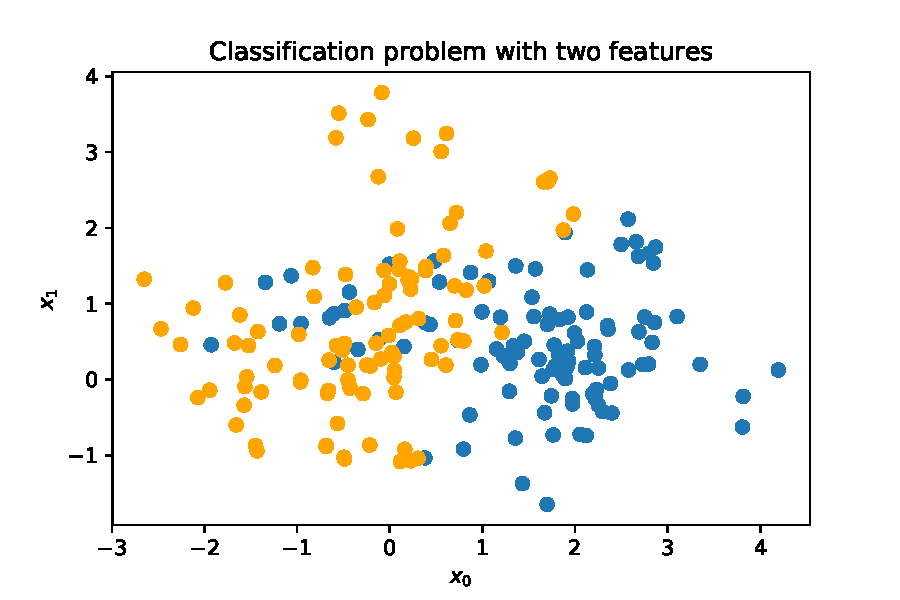
\includegraphics[width=0.5\textwidth]{figures/week_1/classification_problem.pdf}
        \hfill
        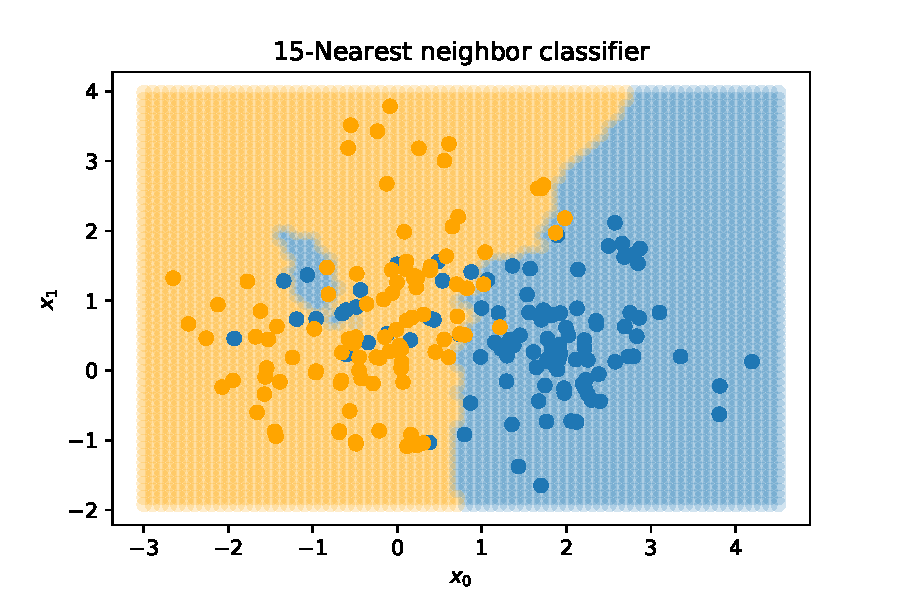
\includegraphics[width=0.5\textwidth]{figures/week_1/15-nn.pdf}
    \end{center}
\end{frame}

\begin{frame}
\frametitle{Linear classifier vs. 15-Nearest neighbour}
    \begin{center}
        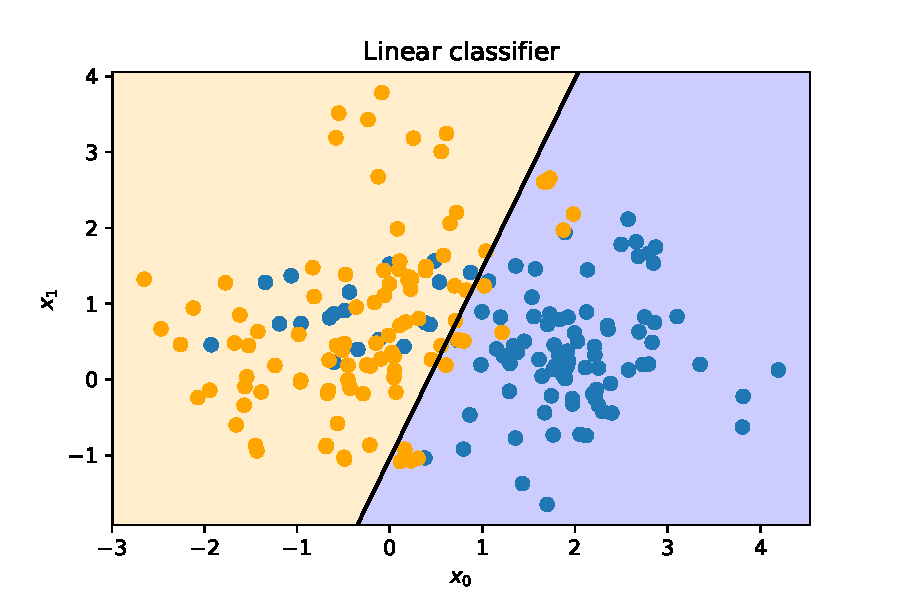
\includegraphics[width=0.5\textwidth]{figures/week_1/linear_model.pdf}
        \hfill
        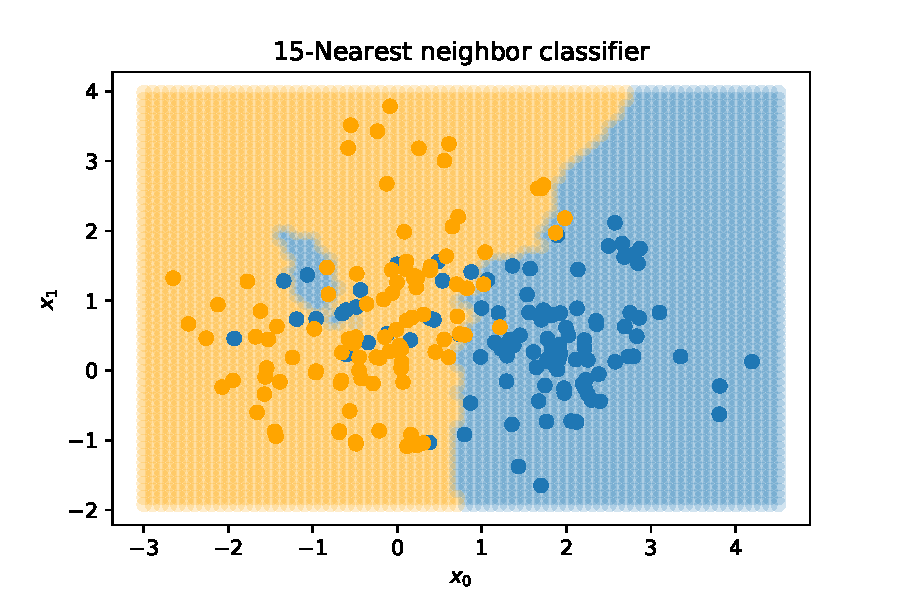
\includegraphics[width=0.5\textwidth]{figures/week_1/15-nn.pdf}
    \end{center}
\end{frame}


\begin{frame}
\frametitle{1-Nearest neighbour vs. 15-Nearest neighbour}
    \begin{center}
        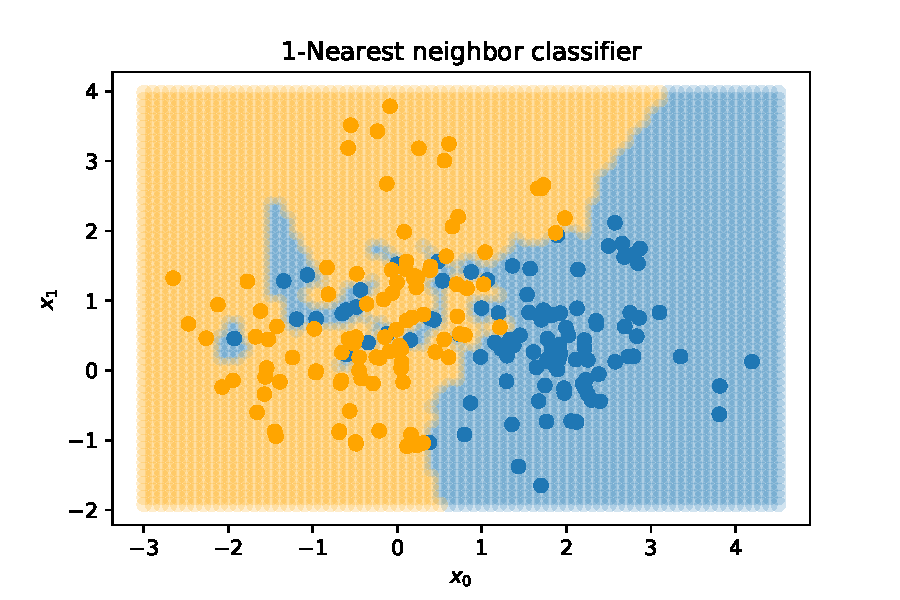
\includegraphics[width=0.5\textwidth]{figures/week_1/1-nn.pdf}
        \hfill
        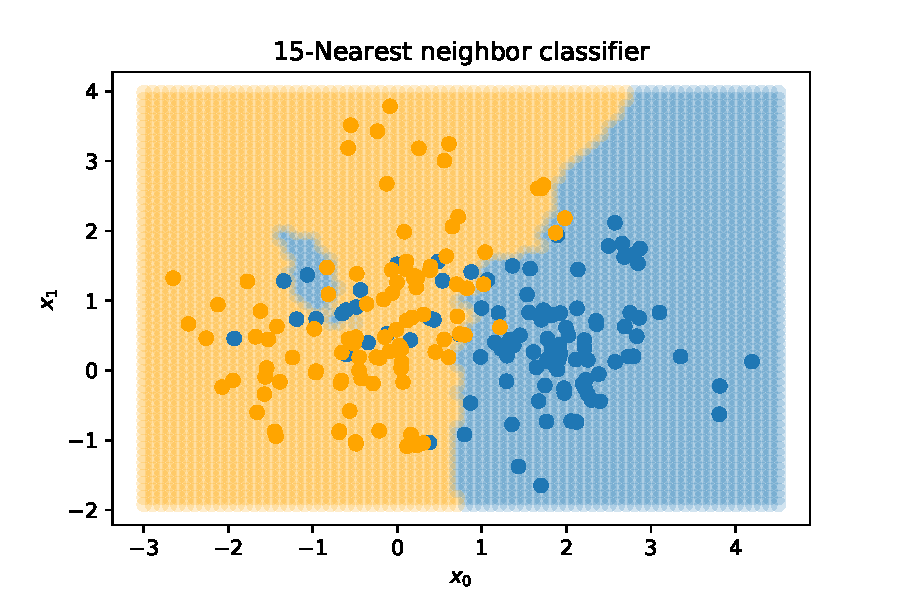
\includegraphics[width=0.5\textwidth]{figures/week_1/15-nn.pdf}
    \end{center}
\end{frame}


\begin{frame}
\frametitle{Comparison of the techniques}
    \begin{itemize}
        \item 15-NN seems to work better than the linear classifier since fewer points are missclassified.
        \item On the other hand, {\bf none} of the points in the 1-NN case was misclassified!?
        \item Actually with the 1-NN method the error on {\bf training data} is always 0.
        \item An independent test set needed to obtain a better comparison of the methods.
    \end{itemize}
\end{frame}

\begin{frame}
\frametitle{Comparison of techniques}

    \begin{itemize}
        \item At first sight it looks like k-NN has only one parameter, $k$ versus $p$ parameters (number of weights $w_i$) of the linear model.
        \item The {\bf effective}  number of parameters of k-NN is $N/k$ which is in general bigger than $p$ ($N$ is the size of the training set).
        \item For instance, assume non-overlapping neighbourhoods
            \begin{itemize}
                \item There will be $N/k$ neighbourhoods.
                \item To each neighbourhood there correspond one parameter (the mean of the elements of the neighbourhood).
            \end{itemize}
    \end{itemize}

\end{frame}


\section{Probability theory}


\begin{frame}
\frametitle{Probability theory}
Materials:
\begin{itemize}
    \item Chapter I.3 from \cite{deeplearning}
\end{itemize}
\end{frame}

\begin{frame}
\frametitle{Probability theory}
\begin{itemize}
    \item Probability theory is a mathematical framework for dealing with uncertainty, i.e., modeling and analyzing uncertain events and statements
    \item In AI probability theory is used in two major ways:
        \begin{itemize}
            \item To design AI systems, i.e., derive models and expressions and the corresponding algorithms.
            \item To analyze the behaviour of the AI systems.
        \end{itemize}

\end{itemize}

\end{frame}

\begin{frame}
\frametitle{Probability theory}
    \begin{itemize}
        \item A {\bf random variable} is a variable that can take values randomly.
        \item We will denote random variables with plain (ordinary text) typeface and their values with standard math typeface\\
        for example, if the random variable is denoted as x its values can be $x_1$ and $x_2$
        \item A vector-valued random variable is denoted with bold typeface, e.g. {\bf x}.
        \item On its own a random variable just denotes the set of its possible values; to get its full meaning in needs to be coupled with a distribution
    \end{itemize}
\end{frame}


\begin{frame}
\frametitle{Probability theory}
    \begin{itemize}
        \item There are two types of random variables: {\bf discrete} and {\bf continuous}.
        \item Consequently there are two ways to describe probability distributions: {\bf probability mass functions} and {\bf probability density functions}.
    \end{itemize}
\end{frame}


\begin{frame}
\frametitle{Probability mass function}
\begin{itemize}
    \item The domain of a probability mass function $P$ is the set of all possible states of the random variable x.
    \item $\forall x \in \text{x}: 0 \leq P(\text(x) \leq 1$
        \begin{itemize}
            \item An impossible event has probability 0 and no state can be less probable than that.
            \item An event that is guaranteed to happen has probability 1 and no state can have a greater chance of occurring.
        \end{itemize}
    \item $\sum_{x \in \text{x}} P(x) = 1$
        \begin{itemize}
            \item We say that \text{x} is {\bf normalized}.
        \end{itemize}
    \item Example: Uniform distribution: $P(\text{x} = x_i) = \frac{1}{k}$.
\end{itemize}
\end{frame}


\begin{frame}
\frametitle{Probability density function}
\begin{itemize}
    \item The domain of the probability density function $p$ must be the set of all possible states of $\text{x}$.
    \item $\forall x \in \text{x}: p(x)\geq 0.$
    \item $$\int p(x)dx = 1$$
    \item Example: uniform distribution $u(x;a,b) = \frac{1}{b-a}$, for $x \in [a,b]$
\end{itemize}

\end{frame}


\begin{frame}
\frametitle{Conditional probability}
    \begin{itemize}
        \item {\bf Conditional probability} is the probability of some event provided that some other event has happened.
        \item
        Given two random variables x and y, the conditional probability that y has value $y$ provided that we know that x has value $x$ is given by
        $$
        P(\text{y}=y \mid \text{x} = x) = \frac{P(\text{x,y})}{P(\text{x}=x)}
        $$
        \item Another way to see this formula is $$P(\text{x,y}) = P(\text{x} = x)P(\text{y} = y \mid \text{x} = x)$$ i.e., the probability of $x$ and $y$ occurring together is equal to the probability of occurrence of $x$ times the probability of $y$ occurring provided $x$ has occurred.
    \end{itemize}

\end{frame}





\begin{frame}
\frametitle{Expectation}
\begin{itemize}
    \item The {\bf expectation} or {\bf expected} value of a function $f(x)$ with respect to a probability distribution $P(x)$ is the average value of $f$ over all values $x$ assuming they are drawn from $P$
    \item $$\field{E}_{\text{x} \sim P} [f(x)] = \sum_{x} P(x) f(x)$$
    \item $$\field{E}_{\text{x} \sim P} [f(x)] = \int p(x) f(x) dx$$
    \item Linarity of expectations:
    $$\field{E}_{\text{x}} [\alpha f(x) + \beta g(x)] =  \alpha \field{E}_\text{x}[f(x)] + \beta \field{E}_\text{x}[g(x)]$$
\end{itemize}

\end{frame}



\begin{frame}
\frametitle{Variance and covariance}
\begin{itemize}
    \item The {\bf variance} gives a measure of variation of the values of a random variable x $$\mbox{Var}(f(x)) = \field{E}[(f(x) - E[f(x)])^2]$$
    Square root of the variance is called {\bf standard deviation}.

    \item The {\bf covariance} is a measure of linear relation as well as scale between $$\mbox{Cov}(f(x),g(x)) = \field{E}[f(x) - E[(f(x)])(g(x) - E[g(x)])]$$
\end{itemize}

\end{frame}


\begin{frame}
\frametitle{Covariance matrix}
    \begin{itemize}
        \item The {\bf covariance matrix} of a random vector $\vect{x} \in \R^n$ is a $n \times n$ matrix with elements
    $$
    \mbox{Cov}(\vect{x})_{i,j} = \mbox{Cov}(x_i,x_j)
    $$
    \item The diagonal elements of the matrix give the variance
    $$
      \mbox{Cov}(\text{x}_i,\text{x}_i) = \mbox{Var}(\text{x}_i)
    $$
    \end{itemize}

\end{frame}



\begin{frame}
\frametitle{Bernouli Distribution}
\begin{itemize}
    \item A distribution over a single binary random variable
    \item Controlled by a single parameter $\phi \in [0,1]$ which corresponds to the probability of the random variable taking the value 1
    \item Properties:
    \begin{eqnarray*}
    P({\rm x}) = 1) = \phi \\
    P({\rm x} = 0) = 1 - \phi \\
    P({\rm x} = x) = \phi^x (1-\phi)^{1-x} \\
    \field{E}_\text{x}[\text{x}] = \phi \\
    Var(\text{x}) = \phi(1-\phi)
    \end{eqnarray*}
\end{itemize}
\end{frame}

\begin{frame}
\frametitle{Gaussian distribution}
\begin{itemize}
    \item The most commonly used distribution, also called {\bf normal distribution}.
    \item Controlled by two parameters $\mu \in \R$ (the {\bf mean}) and $\sigma \in (0, \infty)$, (the {\bf standard deviation})

    $$
    {\cal N}(x ; \mu, \sigma^2) = \sqrt{\frac{1}{2 \pi \sigma^2}} \mbox{exp} \left (-\frac{1}{2 \sigma^2}(x - \mu)^2 \right )
    $$

    $$
    {\cal N}(\vect{x} ; \vect{\mu}, \vect{\Sigma}) = \sqrt{\frac{1}{(2 \pi)^n \mbox{det}(\Sigma)}} \mbox{exp} \left (-\frac{1}{2} (\vect{x} - \vect{\mu})^T \vect{\Sigma}^{-1} (\vect{x} - \vect{\mu}) \right )
    $$


\end{itemize}
\end{frame}


\begin{frame}
\frametitle{Gaussian distribution}
\begin{center}
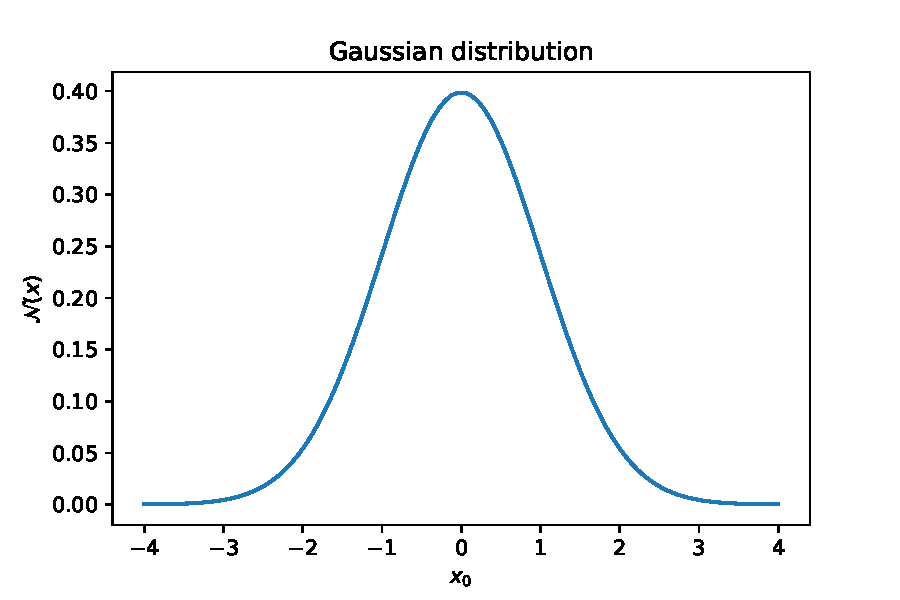
\includegraphics[width=0.5\textwidth]{figures/week_1/gaussian_1d.pdf}
\hfill
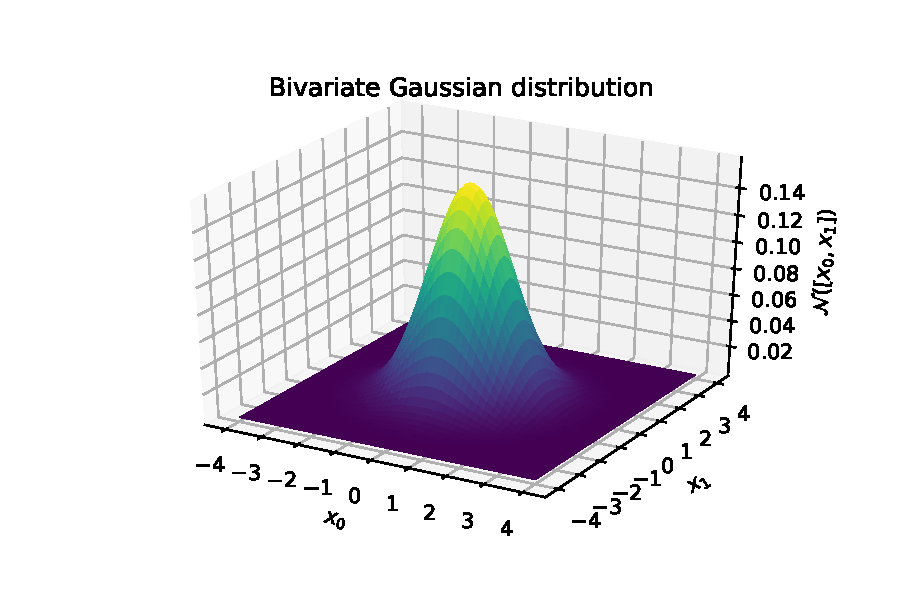
\includegraphics[width=0.5\textwidth]{figures/week_1/gaussian_2d.pdf}
\end{center}
\end{frame}

\begin{frame}
\frametitle{Logistic sigmoid}
\begin{itemize}
    \item A useful function that we are going to consider
    $$\sigma(x) = \frac{1}{1 + \exp{(-x)}}$$
    \item The Logistic (sigmoid) function is commonly used to parametrize Bernoulli distributions.
    \begin{center}
    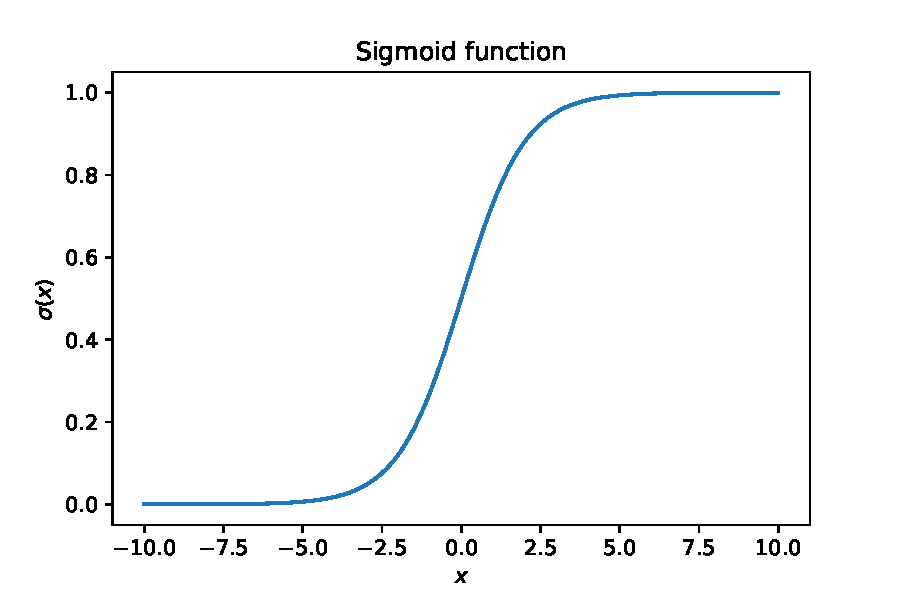
\includegraphics[width=0.5\textwidth]{figures/week_1/sigmoid.pdf}
    \end{center}

\end{itemize}
\end{frame}


\begin{frame}
\frametitle{Bayes' rule}
\begin{itemize}
    \item Suppose know $P(\text{y} \mid \text{x})$, but we actually need $P(\text{x} \mid \text{y})$. If we know $P(\text{x})$ then we can compute
    $$
        P(\text{x} \mid \text{y}) = \frac{P(\text{y} \mid \text{x})P(\text{x})}{P(\text{y})}
    $$
    Although it appears in the formula prior knowledge $P(\text{y}$ is not needed since usually it can be computed as $\sum_{\text{x}} P(\text{y} \mid \text{x})P(\text{x})$
    \item It can be straightforwardly derived from the conditional probability formula.
    \item It could have be named also after Laplace who independently found it, generalized it, and introduced it in practice.
\end{itemize}
\end{frame}


\begin{frame}
\frametitle{Acknowledgements}

The slides for this lecture were prepared by Mitko Veta and Dragan Bo{\v s}nacki. 

Some of the slides are based on the accompanying lectures of \cite{deeplearning}.

\end{frame}


\begin{frame}
\frametitle{References}
\printbibliography
\end{frame}

\end{document}
